\chapter{Общие вопросы}

В этой главе приводятся основные понятия ML и DS. 


\section{Машинное обучение}

Машинное обучение (ML) - область искусственного интеллекта, изучающая самообучающиеся модели, то есть решаюшие поставленную задачу не по заранее запрограммированному алгоритму, а предварительно настраивая свое поведение согласно имеющимся данным. 

Обычно методы ML содержат свободные параметры, подбор которых наилучшим (в смысле имеющихся данных и задачи) образом и составляет процесс обучения алгоритма. После обучения алгоритм можно использовать на новых данных, которые не были представлены алгоритму на стадии обучения.


\section{Основные классы задач}

\subsection{Обучение с учителем}

\subsection{Обучение без учителя}

\subsection{Частичное обучение}

\subsection{Обучение с подкреплением}


\section{Обнаружение аномалий}


\section{Контроль качества}

...оценка обобщающей способности...


\section{Недообучение}


\section{Переобучение}


\section{Регуляризация}


\section{Отбор признаков}


\section{Параметры алгоритма}


\section{Подбора метапараметров}


\section{Основные типы алгоритмов}


\section{Многоклассовая классификация}


\section{Дисбаланс классов}

...чем плохо... как бороться (over/undersampling/SMOTE)...


\section{Ансамбли алгоритмов}

\section{Метрики и функции потерь}

Метрика - величина, обычно диктуемая бизнесом, оптимизация (максимизация или минимизация) которой вполне очевидным образом свидетельствует об улучшении качества работы модели.

Функция потерь - величина, более удобная для оценки/оптимизации модели, уменьшение которой, вообще говоря, приводит к оптимизации метрики задачи.

Иными словами, улучшение метрики - конечная цель процесса обучения алгоритма, но достигается это зачастую оптимизацией именно некоторой функции потерь, с которой может быть удобнее работать.
Метрики и функции потерь - близкие понятия, когда речь идет об оценки качества алгоритма, и их довольно часто смешивают.

\textbf{Пример:} Пусть в задаче бинарной классификации основной метрикой является accuracy - доля правильных ответов. Эта метрика не дифференцируема, поэтому ее оптимизация напрямую методами гладкой оптимизации невозможна. В качестве функции потерь выберем MSE - среднеквадратичную ошибку. Это уже гладкая функция своих аргументов,и ее минимизация скорее всего приведет к увеличению доли правильных ответов, то есть к конечной цели. 

\section{Метрики бинарной классификации}

Пусть некоторый алгоритм $a$ решает задачу бинарной классификации с классами $0$ (негативный) и $1$ (позитивный).
Тестирование алгоритма $a$ проводится на $n$ объектах, ответы $y$ на которых известны. Пусть $TP$ и $TN$ - числа правильно классифицированных позитивных и негативных объектов соответственно. Аналогично, $FP$ и $FN$ - числа неправильно классифицированных позитивных и негативных объектов соответственно.

О качестве алгоритма $a$ можно судить по матрице ошибок:
\begin{center}
\begin{tabular}{ c c c }
     & y=1 & y=0 \\ 
 a=1 & TP  & FP \\  
 a=0 & FN  & TN    
\end{tabular}
\end{center}

Для оценки качества работы алгоритмов бинарной классификации обычно используются описанные далее основные метрики.

\subsection{Accuracy}

Точность (accuracy) - доля правильных ответов,

$$
accuracy = \frac{TP + TN}{n}.
$$

Проста в использовании и интерпретации, но плоха для несбалансированных выборок. Кроме того, не дифференцируема и потому не может быть использована напрямую в качестве функции потерь для алгоритмов гладкой оптимизации.

\subsection{Precision}

Точность (precision) - отношение числа правильно классифицированных позитивных объектов к общему количеству позитивно классифицированных,

$$
precision = \frac{TP}{TP + FP}.
$$

Чем ближе значение к 1, тем меньше ложных срабатываний (FP). Проста в использовании и интуитивна, то не использует информацию о негативно классифицированных объектах и, кроме того, не является дифференцируемой.

\subsection{Полнота (recall)}

Полнота (recall) - вычисляется как отношение

$$
recall = \frac{TP}{TP + FN}.
$$

Чем ближе значение к 1, тем меньше ложных пропусков (FN). Проста в использовании и интуитивна, то не использует TN, FP и, кроме того, не является дифференцируемой.

\subsection{F1-мера}

F1-мера - среднее гармоническое точности и полноты,

$$
F = \frac{2PR}{P + R}.
$$

F1-мера усредняет точность и полноту, является неплохом компромиссом между обеими метриками. Проста в использовании, но плохо интерпретируема и не является дифференцируемой.

\subsection{F-мера}

Обобщенная F-мера вычисляется как

$$
F = (1+\beta^2)\frac{PR}{\beta^2P + R}.
$$

F-мера усредняет точность и полноту, является неплохом компромиссом между обеими метриками, имеет настраиваемый параметр $\beta$. Проста в использовании, но плохо интерпретируема и не является дифференцируемой.

\subsection{ROC кривая}\label{roc-curve}

ROC кривая - характеристика качества алгоритмов бинарной классификации, дающих вероятностноподобный вывод, $a\in[0, 1]$. 
ROC кривая строится в координатах 
$$
FPR = \frac{FP}{FP + TN}, \quad TPR = \frac{TP}{TP + FN}.
$$
Каждая точка кривой - значение $(FPR, TPR)$, полученное для некоторого порога дискретизации алгоритма (см. \ref{pr-curve}). 

Более простой способ построения ROC кривой состоит в следующем:
\begin{enumerate}
    \item отрезки $[0, 1]$ по осям $TPR$ и $FPR$ разбиваются на $\#[y=0]$ и $\#[y=1]$ частей соответственно.
    \item пары реальных ответов $y_i$ упорядочиваются по убыванию соответствующих ответов алгоритма $a_i$.
    \item проходя по получившемуся после сортировки массиву значений $y_i$, строим ROC кривую, начиная от начала координат и делая шаг вправо, если $y_i=0$ и вверх, если $y_i=1$. Важный момент: если рядом по порядку оказались несколько $a_i$ с одинаковыми значениями, то соответствующий им участок ROC кривой будет не ступенчатым, а прямолинейным (см. пример ниже).
\end{enumerate}

ROC кривая идеального алгорима проходит через точки $(0,0)$, $(0,1)$, $(1,1)$; для случайного гадания - проходит вблизи прямой $FPR = TPR$. Наилучшим значением порога дискретизации алгоритма может считаться порог, соответствующий точке на ROC кривой, ближайшей к $(0, 1)$, либо точке, наиболее удаленной от прямой случайного гадания $TPR = FPR$. 

\textbf{Пример:} для алгоритма, дающего вывод как в таблице ниже, график $ROC$ кривой выглядит следующим образом

\begin{tabular}{ c c }
    \raisebox{-\totalheight}{
    \begin{tabular}{|c|c|c|c|c|c|c|c|} 
        \hline
        y & 1 & 0 & 0 & 1 & 0 & 1 & 0 \\ 
        \hline
        a & 1.0 & 0.9 & 0.9 & 0.9 & 0.8 & 0.3 & 0.2 \\
        \hline
    \end{tabular}}
    & 
    \raisebox{-\totalheight}{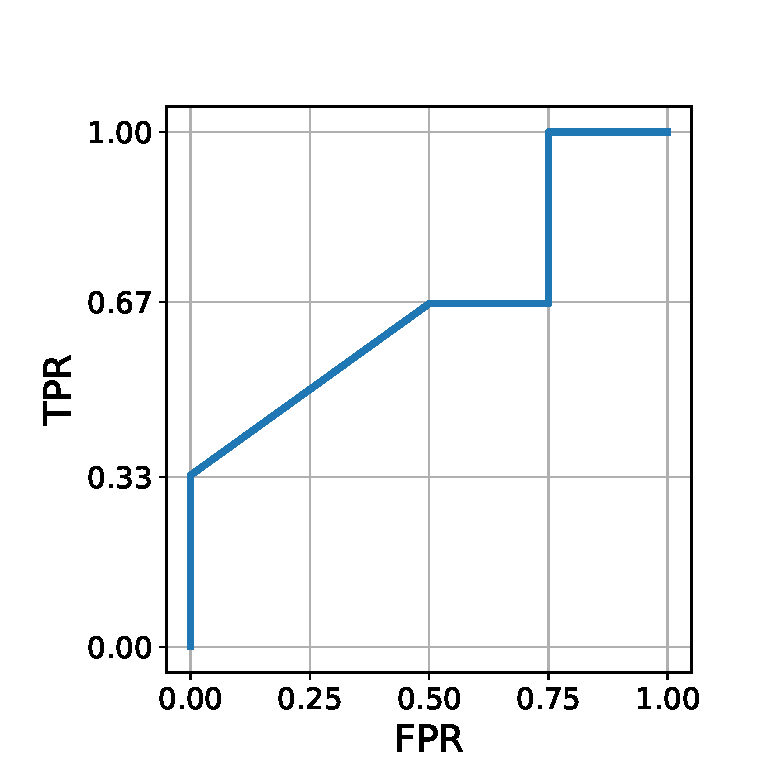
\includegraphics[scale=0.4]{images/roc-curve.eps}}
\end{tabular}

\subsection{ROC-AUC}

ROC-AUC - площадь под ROC кривой. Применяется к алгоритмам бинарной классификации, дающим вероятностноподобный вывод, $a\in[0, 1]$, позволяя оценить алгоритм "в целом", без привязки к конкретному значению порога дискретизации алгоритма.

ROC-AUC принимает значения от $0$ до $1$. Значения близкие к $0.5$ интерпретируются как самые худшие (случайное гадание), близкие к $1$ - как хорошие. ROC-AUC более устойчива к дисбалансу классов, чем Accuracy, но не так хорошо, как PR-AUC. ROC-AUC также не учитывает уверенность алгоритма в своих предсказаниях (насколько близко распределены предсказания к $0$ и $1$). Не является дифференцируемой.

ROC-AUC для примера \ref{roc-curve} равна $2/3$.

\subsection{PR кривая}\label{pr-curve}

PR кривая - характеристика качества алгоритмов бинарной классификации, дающих вероятностноподобный вывод, $a\in[0, 1]$. 
PR кривая строится в координатах 
$$
recall = \frac{TP}{TP + FN}, \quad precision = \frac{TP}{TP + FP}.
$$
Каждая точка кривой - значение $(recall, precision)$, полученное для некоторого порога дискретизации алгоритма. 

Способ построения PR кривой состоит в следующем:
\begin{enumerate}
    \item вычисляются пороги $h$ - всевозможные значения ответов алгоритма $a$.
    \item ответы $a_i$ дискретизируются для каждого значения порога и вычисляются значения $recall$ и $precision$. При этом ордината первой точки кривой, соответствующей порогу $h>1$, не определена, так как знаменатель $precision$ обращается в ноль. В качестве ординаты берется ордината второй точки.
    \item по полученным точкам строится график PR кривой. 
\end{enumerate}

PR кривая идеального алгорима проходит через точки $(0,1)$, $(1,1)$, $(1,\#[y=1]/n)$; для случайного гадания - проходит вблизи прямой $precision = \#[y=1]/n$.

\textbf{Пример:} для алгоритма, дающего вывод как в таблице ниже, график $PR$ кривой выглядит следующим образом

\begin{tabular}{ c c }
    \raisebox{-\totalheight}{
    \begin{tabular}{|c|c|c|c|c|c|c|c|} 
        \hline
        y & 1 & 0 & 0 & 1 & 0 & 1 & 0 \\ 
        \hline
        a & 1.0 & 0.9 & 0.9 & 0.9 & 0.8 & 0.3 & 0.2 \\
        \hline
    \end{tabular}}
    & 
    \raisebox{-\totalheight}{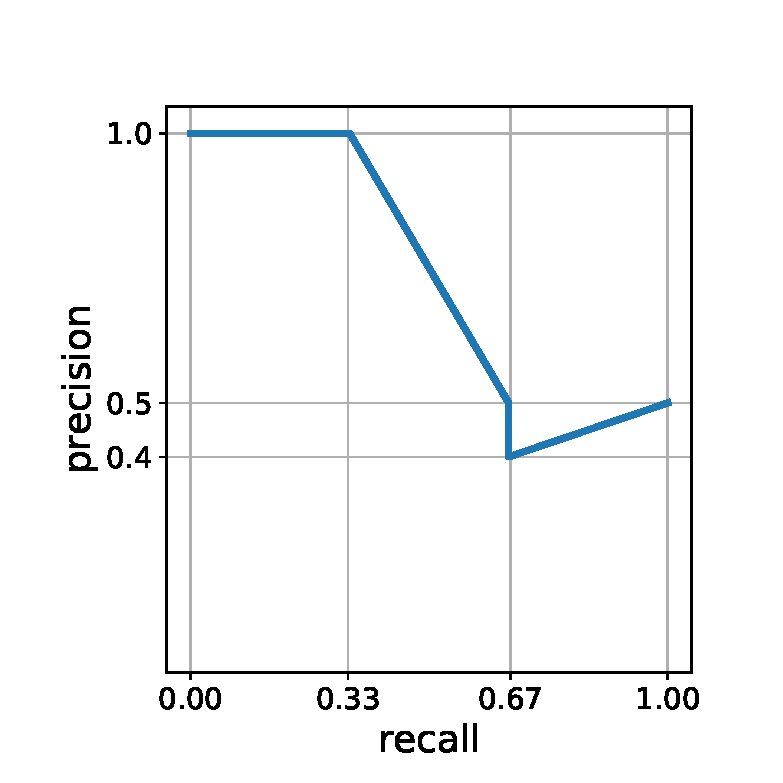
\includegraphics[scale=0.4]{images/pr-curve.eps}}
\end{tabular}

\subsection{PR-AUC}

PR-AUC - площадь под PR кривой. Применяется к алгоритмам бинарной классификации, дающим вероятностноподобный вывод, $a\in[0, 1]$, позволяя оценить алгоритм "в целом", без привязки к конкретному значению порога дискретизации алгоритма.

PR-AUC - площадь под PR кривой. Принимает значения от $0$ до $1$. Значения близкие к $1$ интерпретируются как хорошие, близкие к $\#[y=1]/n$ - как самые худшие (случайные гадания). PR-AUC более устойчива к дисбалансу классов, чем ROC-AUC, однако, не учитывает уверенность алгоритма в своих предсказаниях (насколько близко распределены предсказания к $0$ и $1$). Не является дифференцируемой.

PR-AUC для примера \ref{pr-curve} равна $11/15\approx 0.73$.

\subsection{Бинарная кросс-энтропия (logloss)}

Пусть $y$ - истинная метка объекта ($0$ или $1$), а $a$ - ответы некоторого алгоритма (число из $[0, 1]$). Бинарная кросс-энтропия (logloss) вычисляется как
$$
L(y, a) = -y\log_2 a - (1-y)\log_2(1-a).
$$
Слагаемые с нулевым множителем при логарифме (соответствующие $y=0$ и $y=1$) полагаются равными нулю.

Полная кросс-энтропия на множестве ответов определяется усреднением значений по всем объектам.

Бинарная кросс-энтропия имеет следующую вероятностную интерпретацию. Пусть метка $i$-му объекту назначается по схеме Бернулли, т.е. метка полагается равной $y_i=1$ с вероятностью $a_i$ и $y_i=0$ с вероятностью $1-a_i$. Тогда вероятность получить истинные ответы $y_i$ равна
$$
\prod_{i=1}^na_i^{y_i}(1-a_i)^{1-y_i}.
$$
Логарифмируя, получаем правдоподобие, совпадающее с бинарной кросс-энтропией с точностью до знака. Таким образом, нахождение ответов $a_i$ с позиции минимизации бинарной кросс-энтропии равносильно максимизации правдоподобия.


https://en.wikipedia.org/wiki/Loss_functions_for_classification


\section{Метрики многоклассовой классификации}

\subsection{Категориальная кросс-энтропия (logloss)}


\section{Индекс Джини}


\section{Метрики регрессии}

\subsection{Среднеквадратичная ошибка (MSE)}

Пусть $y$ - истинная метка объекта ($0$ или $1$), а $a$ - ответы некоторого алгоритма (число из $[0, 1]$). Среднеквадратичная ошибка вычисляется как
$$
L(y, a) = (y - a)^2.
$$

Полная cреднеквадратичная ошибка на множестве ответов определяется усреднением значений по всем объектам.
Наилучшим константным предсказанием для MSE является выборочное среднее:
$$
a = \frac{1}{n}\sum_{i=1}^ny_i
$$

MSE дифференцируема и проста в использовании, но плохо интрепретируема, так как дает ненормированный ни к чему результат, который трудно с чем-либо сравнить. Кроме того, MSE чувствительна к выбросам в выборке.

\subsection{Среднеабсолютная ошибка (MAE)}

Пусть $y$ - истинная метка объекта ($0$ или $1$), а $a$ - ответы некоторого алгоритма (число из $[0, 1]$). Среднеабсолютная ошибка вычисляется как
$$
L(y, a) = |y - a|.
$$

Полная cреднеквадратичная ошибка на множестве ответов определяется усреднением значений по всем объектам.
Наилучшим константным предсказанием для MSE является выборочная медиана.

MAE проста в использовании, но недифференцируема и плохо интрепретируема, так как дает ненормированный ни к чему результат, который трудно с чем-либо сравнить. MAE менее чувствительна к выбросам в выборке, чем MSE.


\section{Метрики кластеризации}


\section{Разложение ошибки алгоритма}


\section{Кривые валидации}


\section{Кривые обучения}


\section{Метрические методы}


\section{Метод ближайших соседей}


\section{Линейные методы}


\section{Линейная регрессия}


\section{Логистическая регрессия}

...отличие от линейной...


\section{SVM}


\section{Ядра и спрямляющие пространства}


\section{Решаюшие деревья}


\section{Случайный лес}

...отличие от беггинга над решающими деревьями...


\section{Градиентный бустинг}


\section{Байесовские методы}



